\documentclass[11pt]{article}
\usepackage[margin=1in]{geometry}
\usepackage{amsmath,amssymb}
\usepackage{booktabs}
\usepackage{tikz}
\usetikzlibrary{shapes.geometric,arrows.meta,positioning}
\usepackage{pgfplots}
\pgfplotsset{compat=1.9}
\usepackage[colorlinks=true,linkcolor=blue,citecolor=blue,urlcolor=blue]{hyperref}

\title{A Receipt-First Estate: Honest Operational Accounting of a Governed AI Research Organization\\ \large November 2026 Census Edition}
\author{Stephen P.\ Lutar Jr.\\ SZL Holdings, Inc.\\ \texttt{ORCID 0009-0001-0110-4173}}
\date{November 15, 2026}

\begin{document}
\maketitle

\begin{abstract}
This report is an operational accounting of a governed AI research estate --- the SZL Holdings organization --- written under a receipt-first doctrine in which every measured claim is bound to a dated, addressable artifact (a repository commit, an API-observable receipt file, or a DOI-minted record), and every unmeasured claim is labeled as such. The estate comprises a GitHub organization of 159 repositories, a Hugging Face organization whose public face on the census date exposes 131 models, 71 datasets, and 32 Spaces through the anonymous API, a Lean~4/Mathlib proof corpus with a locked registry of exactly eight machine-checked formulas, and an on-chain receipt substrate exceeding one thousand receipt files. We report: (i) continuous-integration health of 121 of 130 active repositories green at last run; (ii) a full-corpus proof-attempt campaign of 143/143 attempts with 65 honestly recorded \texttt{sorry}-echo failures and zero fabrications; (iii) an evaluation battery whose most recent binding wave scores 37 of 41 bindings at 0/6 with disclosed abstention failures --- reported as the headline finding it is, not smoothed; (iv) receipt-gated corpus admission measured at 2.67\%, 1.33\%, 20.67\%, and 21.90\% across four gates with per-row denominators published; and (v) a disclosed incident in which a marketing-stamping job overwrote 138 public model cards and was repaired by byte-exact, commit-addressed restoration. Every figure in this paper is generated from data read on November 14--15, 2026, from live APIs or on-disk logs, and the provenance of each figure is tabulated in the appendix. The paper claims operational honesty, not scientific novelty: no benchmark here is state-of-the-art, several measured results are failures, and the contribution is the accounting discipline itself.
\end{abstract}

\section{Introduction and Doctrine}
\label{sec:intro}

Agentic AI organizations face an accounting problem before they face a science problem. When a research estate produces models, datasets, proofs, deployments, and publications at machine speed, the binding constraint on trust is not the production rate but the \emph{verifiability rate}: the fraction of claims whose evidence can be re-read by a third party at a stable address. This report describes an estate built around one constraint: \textbf{no claim without a receipt}.

The doctrine has three tiers, applied uniformly:
\begin{itemize}
\item \textbf{MEASURED}: a dated artifact (receipt file, API record, CI run) at a stable address backs the claim.
\item \textbf{UNKNOWN}: no artifact exists; the claim is explicitly not made.
\item \textbf{ABSTAIN}: an artifact exists and records a failure or a refusal to answer; the failure is published as a first-class result.
\end{itemize}

The tiers exist because the failure mode of agentic research organizations is not lying but \emph{drift}: a claim that was once measured survives into contexts where its measurement no longer applies, and a card that was once honest accumulates language faster than evidence. A three-tier discipline makes drift detectable --- an unmeasured claim is not merely weak, it is \emph{noncompliant} with the estate's own published standard, and any reader can cite the tier against it. The tiers also price honesty correctly: ABSTAIN results cost publication prestige but buy the only currency that compounds --- a reader who has seen the estate publish its failures has a reason to believe its successes.

Under this doctrine a 0/6 evaluation score is not an embarrassment to be buried; it is a receipt. Section~\ref{sec:battery} reports exactly such a wave. The estate's public interfaces are: the GitHub organization \texttt{szl-holdings} (159 repositories), the Hugging Face organization \texttt{SZLHOLDINGS} (public census in Section~\ref{sec:census}), the Lean~4 proof corpus at the frozen repository \texttt{szl-holdings/lutar-lean}, and the receipt datasets described in Section~\ref{sec:substrate}. Two companion papers --- one on machine-checked append-only governance (25 pages) and one on a graph-shaped audit of governance aggregation (26 pages) --- carry the formal content; this report is the operational layer beneath them: what exists, what is green, what failed, and where every number lives.

\paragraph{Scope and honesty boundary.} This is not a survey of scientific results. It is an operational census. Numbers are point-in-time (November 14--15, 2026), API-observable, and reproducible by the commands in Section~\ref{sec:repro}. Where the estate failed, the failure is printed with the same typography as the successes.

\paragraph{How to read this paper.} Sections~\ref{sec:census}--~\ref{sec:lean} are the census layer: what exists and how healthy it is. Sections~\ref{sec:tracka}--~\ref{sec:battery} are the measurement layer: the two flagship honesty instruments, both reported with their failures exposed. Sections~\ref{sec:cards}--~\ref{sec:deploy} are the case-study layer: integrity, delivery, and a gate series with per-row denominators. Section~\ref{sec:incident} is the incident record at full length. Sections~\ref{sec:loop}--~\ref{sec:change} are the operating layer, and Sections~\ref{sec:limits}--~\ref{sec:concl} state what the paper does not claim. A reader with ten minutes should read the abstract, Figure~\ref{fig:battery}, Table~\ref{tab:gates}, and Section~\ref{sec:incident}; the rest is the audit trail.

\section{Estate Census}
\label{sec:census}

\subsection{GitHub organization}
The GitHub organization \texttt{szl-holdings} holds \textbf{159 repositories} (25 private, 29 archived at census time). The active-repo language profile is dominated by Python, with TypeScript, HTML/JS, Lean (\texttt{lutar-lean}), TeX (\texttt{szl-papers}), and CSS as secondary families. The two paper-bearing repositories are \texttt{szl-papers} (LaTeX sources, preprint metadata, DOI registry) and \texttt{lutar-lean} (Lean~4/Mathlib proof corpus and its attempt receipts). The repositories of record referenced throughout this paper are listed in Table~\ref{tab:repos}.

\begin{table}[htbp]
\centering
\small
\begin{tabular}{lp{8.8cm}}
\toprule
\textbf{Repository} & \textbf{Role} \\
\midrule
\texttt{szl-papers} & Paper sources, preprint metadata, DOI registry (this report included). \\
\texttt{lutar-lean} & Lean~4/Mathlib proof corpus, locked registry, attempt receipts. \\
\texttt{szl-forge} & Delivery pipeline: model-card governance, publisher workflows, CI frontier checks. \\
\texttt{a11oy} & Live estate application; main HEAD mirrored by the honest-status endpoint. \\
\texttt{szl-safe-stack} & Safety-stack components (carries the disclosed CI deadlock of \S\ref{sec:ci}). \\
\texttt{platform} & Estate platform services. \\
\texttt{szl-org-health} & Organization health automation (merge receipts of \S\ref{sec:change}). \\
\texttt{SZLHOLDINGS/frontier-54-runs} & Receipt substrate dataset (\S\ref{sec:substrate}). \\
\texttt{SZLHOLDINGS/lean-proof-corpus-v1} & Proof-corpus dataset with the 143 Track A attempt receipts. \\
\bottomrule
\end{tabular}
\caption{Repositories of record for this census. Every figure in this paper reads from one of these addresses.}
\label{tab:repos}
\end{table}

\subsection{Hugging Face organization}
The anonymous public API on the census date returns:
\begin{center}
\begin{tabular}{lrl}
\toprule
\textbf{Artifact} & \textbf{Public count} & \textbf{Endpoint} \\
\midrule
Models & 131 & \texttt{/api/models?author=SZLHOLDINGS} \\
Datasets & 71 & \texttt{/api/datasets?author=SZLHOLDINGS} \\
Spaces & 32 & \texttt{/api/spaces?author=SZLHOLDINGS} \\
\bottomrule
\end{tabular}
\end{center}
The 32 public Spaces include the estate's live application surfaces --- the showcase, the estate's primary Space, and the organization card --- which the probe sweep of Section~\ref{sec:edge} returns HTTP 200 for. These are \emph{anonymous} counts: privately held repositories (45 models at the November 14 audit) are not visible to the unauthenticated endpoint and are excluded here rather than estimated. An earlier authenticated audit recorded 183 model repositories including private ones; that figure is not re-claimed here because the census instruments differ. The private vault (45 model repositories at the November 14 audit) is composed of laptop-LoRA mirrors, enterprise candidates, organization placeholders, and triage-stage candidates; exposure is contained by privacy, and the same fail-closed card rules govern it --- the audit found all 45 carried the same wave-4 stamp signature and none is claimed as measured here. Figure~\ref{fig:census} shows the public census.

\begin{figure}[htbp]
\centering
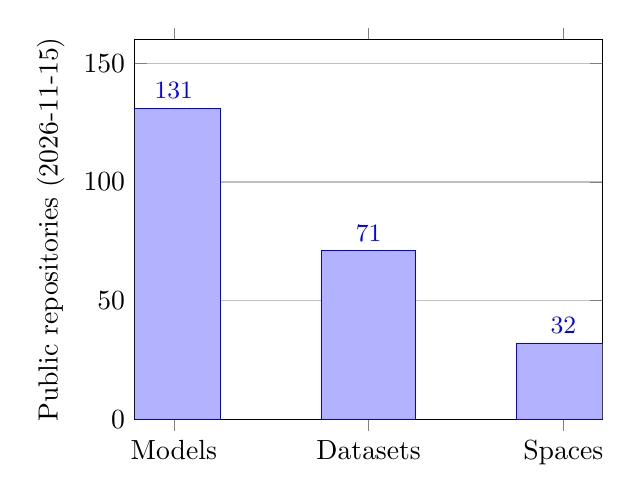
\begin{tikzpicture}
\begin{axis}[
  ybar, bar width=34pt,
  width=0.62\textwidth, height=6.4cm,
  symbolic x coords={Models, Datasets, Spaces},
  xtick=data, ymin=0, ymax=160,
  ylabel={Public repositories (2026-11-15)},
  nodes near coords, every node near coord/.append style={font=\small},
  ymajorgrids=true,
]
\addplot coordinates {(Models,131) (Datasets,71) (Spaces,32)};
\end{axis}
\end{tikzpicture}
\caption{Public Hugging Face census, anonymous API, November 15, 2026. Private repositories are excluded by instrument, not by choice.}
\label{fig:census}
\end{figure}

\subsection{The vertical map}
The estate is organized as twelve research verticals. Figure~\ref{fig:verticals} maps them with their census status. Each vertical's claims live in its own repositories and receipt namespaces; none of the twelve is claimed to be complete, and two (Clinical/Transport Observability, Creativity) are explicitly early-stage with artifact-honest cards only.

\begin{figure}[htbp]
\centering
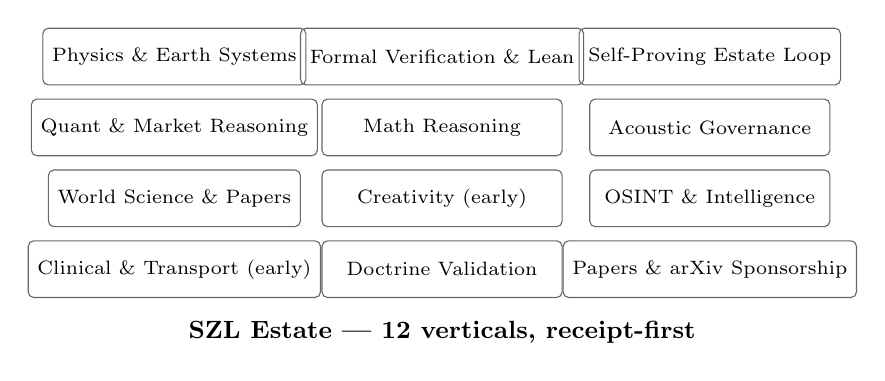
\begin{tikzpicture}[
  box/.style={draw=black!60, rounded corners=2pt, align=center, font=\scriptsize, minimum width=3.05cm, minimum height=0.72cm},
]
\node[box] (p) at (0,3.0) {Physics \& Earth Systems};
\node[box] (l) at (3.4,3.0) {Formal Verification \& Lean};
\node[box] (s) at (6.8,3.0) {Self-Proving Estate Loop};
\node[box] (q) at (0,2.1) {Quant \& Market Reasoning};
\node[box] (m) at (3.4,2.1) {Math Reasoning};
\node[box] (a) at (6.8,2.1) {Acoustic Governance};
\node[box] (w) at (0,1.2) {World Science \& Papers};
\node[box] (c) at (3.4,1.2) {Creativity (early)};
\node[box] (o) at (6.8,1.2) {OSINT \& Intelligence};
\node[box] (t) at (0,0.3) {Clinical \& Transport (early)};
\node[box] (d) at (3.4,0.3) {Doctrine Validation};
\node[box] (x) at (6.8,0.3) {Papers \& arXiv Sponsorship};
\node[draw=none, font=\small\bfseries] at (3.4,-0.5) {SZL Estate --- 12 verticals, receipt-first};
\end{tikzpicture}
\caption{The twelve-vertical estate map as tracked on the internal frontier board. Two verticals are marked early-stage; no vertical is claimed complete.}
\label{fig:verticals}
\end{figure}

\section{Continuous Integration Health}
\label{sec:ci}

The CI census reads the last workflow run per repository. Of 130 active repositories:
\begin{itemize}
\item \textbf{121} last-run \texttt{success};
\item \textbf{1} \texttt{action\_required} (a review-gated repository whose required check is a dead protection context --- an owner-action deadlock, documented, not bypassed);
\item \textbf{2} transient (\texttt{pending}/\texttt{in\_progress} at read time);
\item \textbf{6} \texttt{NO\_RUNS} (three repositories with no workflows by design --- a backup repository, a sandbox, and an acoustic research repository --- and three GHSA advisory placeholders).
\end{itemize}
The \texttt{action\_required} case deserves its own sentence: the repository's branch protection references a required check that no longer exists on any workflow path (a dead protection context), so every run ends awaiting an owner action that no automation may perform. The doctrine-correct treatment is exactly this paragraph --- a deadlock published in a census, not a protection gate quietly dropped to turn the census green. Zero repositories were disabled manually. Figure~\ref{fig:ci} shows the distribution. The single \texttt{action\_required} case is reported here precisely because the estate's doctrine forbids silently bypassing a protection gate to turn a red census green: the deadlock itself is the receipt.

\begin{figure}[htbp]
\centering
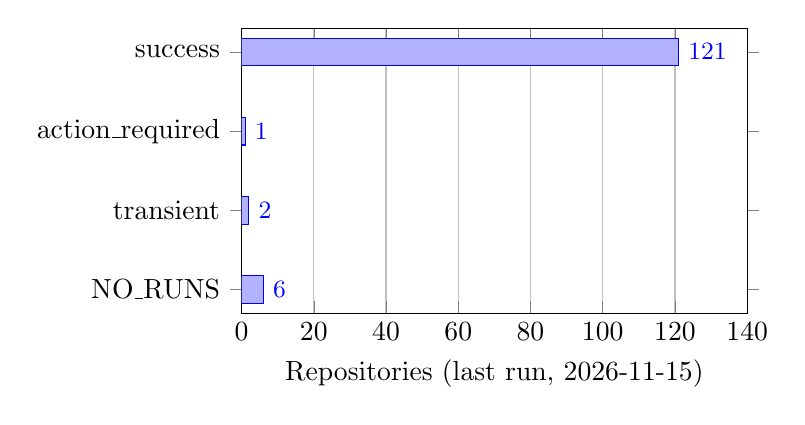
\begin{tikzpicture}
\begin{axis}[
  xbar, width=0.66\textwidth, height=5.2cm,
  symbolic y coords={NO\_RUNS, transient, action\_required, success},
  ytick=data, xmin=0, xmax=140,
  xlabel={Repositories (last run, 2026-11-15)},
  nodes near coords, every node near coord/.append style={font=\small},
  ymajorgrids=false, xmajorgrids=true,
]
\addplot coordinates {(121,success) (1,action\_required) (2,transient) (6,NO\_RUNS)};
\end{axis}
\end{tikzpicture}
\caption{CI health of the 130 active repositories. The action\_required deadlock is disclosed rather than bypassed.}
\label{fig:ci}
\end{figure}

\section{The Receipt Substrate}
\label{sec:substrate}

The estate's receipts live in versioned Hugging Face datasets, addressed by repository and commit. The largest receipt dataset, \texttt{SZLHOLDINGS/frontier-54-runs}, exposes more than one thousand files through the tree API (which caps at 1000 entries; the true count is at least the cap). Table~\ref{tab:namespaces} and Figure~\ref{fig:namespaces} give the namespace distribution at census time.

\begin{table}[htbp]
\centering
\small
\begin{tabular}{lr}
\toprule
\textbf{Namespace} & \textbf{Files} \\
\midrule
\texttt{mesh/} (GPU-worker run receipts) & 872 \\
\texttt{benchmark/} (evaluation batteries) & 67 \\
\texttt{collaboration/} (co-signed instruments) & 11 \\
\texttt{deploy/} & 10 \\
\texttt{doctrine/} & 7 \\
\texttt{receipts/} (dated sweep receipts) & 7 \\
\texttt{lean/} & 6 \\
\texttt{census/} & 5 \\
\texttt{competitive/}, \texttt{wheels/}, \texttt{data/}, \texttt{energy/} & 2 each \\
\texttt{tools/}, \texttt{officers/}, \texttt{monetization/}, \texttt{registry/}, \texttt{proving-ground/} & 1 each \\
\midrule
\textbf{Total (API-capped)} & \textbf{$\geq$1000} \\
\bottomrule
\end{tabular}
\caption{Namespace distribution of \texttt{frontier-54-runs} on 2026-11-15. The tree API returns at most 1000 entries; the mesh namespace dominates because every GPU worker checkpoint writes a receipt.}
\label{tab:namespaces}
\end{table}

\begin{figure}[htbp]
\centering
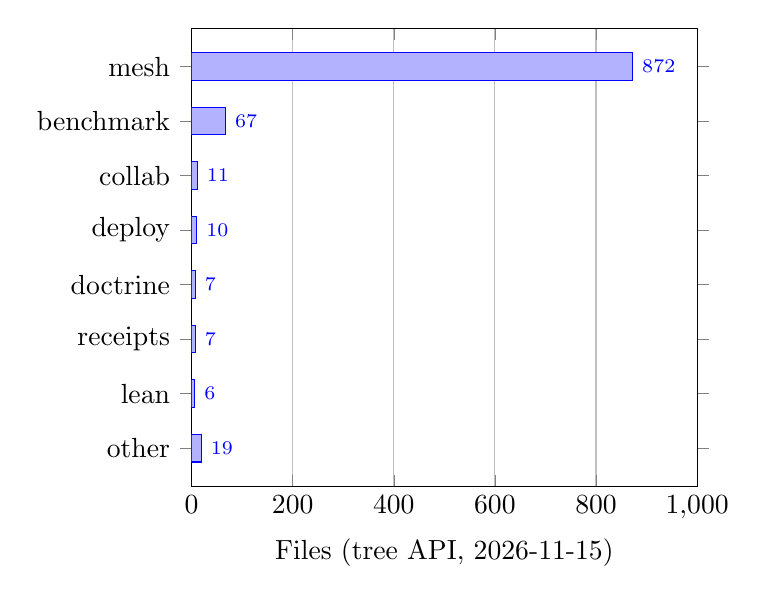
\begin{tikzpicture}
\begin{axis}[
  xbar, width=0.66\textwidth, height=7.4cm,
  symbolic y coords={other, lean, receipts, doctrine, deploy, collab, benchmark, mesh},
  ytick=data, xmin=0, xmax=1000,
  xlabel={Files (tree API, 2026-11-15)},
  nodes near coords, every node near coord/.append style={font=\scriptsize},
  xmajorgrids=true,
]
\addplot coordinates {(872,mesh) (67,benchmark) (11,collab) (10,deploy) (7,doctrine) (7,receipts) (6,lean) (19,other)};
\end{axis}
\end{tikzpicture}
\caption{Receipt distribution by namespace (\textquotedblleft other\textquotedblright{} aggregates the sub-10 namespaces). The mesh namespace's 872 receipts are per-worker-run records from the SaladCloud GPU lanes.}
\label{fig:namespaces}
\end{figure}

Eight Zenodo DOIs pin the preprint lineage (the umbrella record is \texttt{10.5281/zenodo.19944926}); the DOI registry lives in \texttt{szl-papers} and a consistency checker enforces that every README claiming a measured section carries a live deposit.

\section{Formal Verification: The Lean 4 Corpus}
\label{sec:lean}

The proof corpus \texttt{szl-holdings/lutar-lean} is a Lean~4/Mathlib project whose disclosure discipline separates three registries that are easy to conflate and fatal to conflate publicly:
\begin{enumerate}
\item the \textbf{locked-proven formula registry}, which moved from five to exactly eight entries (\texttt{locked\_count\_eight}, proved \texttt{by decide}), containing the focal governance invariants F1, F4, F7, F11, F12, F18, F19, F22;
\item the \textbf{canonical declaration baseline} 749/14/163 (theorems/definitions/instances) frozen at the earlier doctrine commit \texttt{c7c0ba17} --- a distinct object from the proof snapshot;
\item the \textbf{proof snapshot} \texttt{5cfaf9a3} at which the three newest invariants (F4 acyclicity preserved under append, F7 FIFO batch drain with positional equality witness, F22 strictly monotone emit log) are kernel-checked and non-vacuous.
\end{enumerate}

The corpus ledger at the audited commit records 12 declarations in the audit-workflow set, 5 in the pipeline set, and 8 in the locked set (Figure~\ref{fig:ledger}); per-classifier witness-class counting records $\varnothing$=7, $\{P\}$=4, $\{P,Q\}$=1, $\{P,C,Q\}$=13 (Figure~\ref{fig:verdict}), with final verdicts 3 confirmed, 2 conditional, 2 refined, 1 held.

\begin{figure}[htbp]
\centering
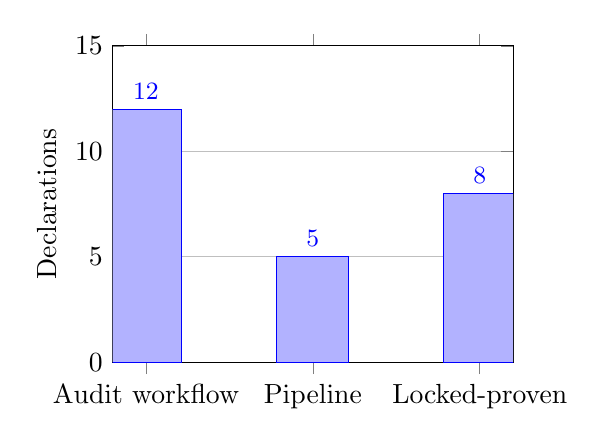
\begin{tikzpicture}
\begin{axis}[
  ybar, bar width=26pt,
  width=0.55\textwidth, height=5.6cm,
  symbolic x coords={Audit workflow, Pipeline, Locked-proven},
  xtick=data, ymin=0, ymax=15,
  ylabel={Declarations},
  nodes near coords, every node near coord/.append style={font=\small},
  ymajorgrids=true,
]
\addplot coordinates {(Audit workflow,12) (Pipeline,5) (Locked-proven,8)};
\end{axis}
\end{tikzpicture}
\caption{Declaration ledger by registry at the audited corpus commit. The locked-proven set is exactly eight; the count is machine-checked (\texttt{locked\_count\_eight}, \texttt{by decide}).}
\label{fig:ledger}
\end{figure}

\begin{figure}[htbp]
\centering
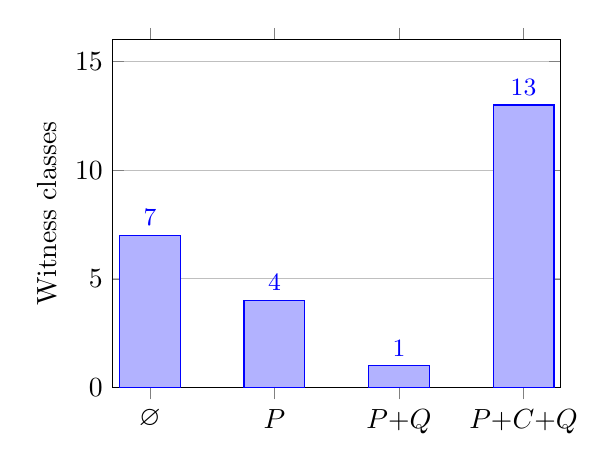
\begin{tikzpicture}
\begin{axis}[
  ybar, bar width=22pt,
  width=0.6\textwidth, height=6.0cm,
  symbolic x coords={none, P, PQ, PCQ},
  xtick=data, ymin=0, ymax=16,
  xticklabels={$\varnothing$, $P$, $P{+}Q$, $P{+}C{+}Q$},
  ylabel={Witness classes},
  nodes near coords, every node near coord/.append style={font=\small},
  ymajorgrids=true,
]
\addplot coordinates {(none,7) (P,4) (PQ,1) (PCQ,13)};
\end{axis}
\end{tikzpicture}
\caption{Witness-class distribution over the audited declaration set ($P$ = proof term, $Q$ = qualifier, $C$ = constructor evidence). The mass in $\{P,C,Q\}$ reflects the non-vacuity audit: a bare proof term without constructor evidence is not admitted to the registry.}
\label{fig:verdict}
\end{figure}

\subsection{The locked invariants}
The eight-entry locked registry (F1, F4, F7, F11, F12, F18, F19, F22) is maintained as a \emph{diffable} object: the canonical declaration baseline (749 theorems / 14 definitions / 163 instances) was frozen at doctrine commit \texttt{c7c0ba17} \emph{before} the registry grew from five to eight entries, so the growth is auditable as a diff against a frozen denominator rather than a re-baseline. The three newest members of the registry are representative of the corpus's subject matter --- append-only governance data structures:
\begin{itemize}
\item \textbf{F4}: acyclicity of the governance trace DAG is preserved under append (the append operation cannot create a cycle);
\item \textbf{F7}: the FIFO batch drain admits a positional equality witness (draining a batch preserves the order in which entries were admitted);
\item \textbf{F22}: the emit log is strictly monotone (emitted sequence numbers strictly increase).
\end{itemize}
Each invariant is kernel-checked at snapshot \texttt{5cfaf9a3} and each carries the non-vacuity evidence of Figure~\ref{fig:verdict}: a bare proof term without constructor evidence is not admitted to the registry. The registry count itself is machine-checked (\texttt{locked\_count\_eight}, \texttt{by decide}) --- the paper's claim is not that the list above is complete but that the machine's count is the authority.

\subsection{Training receipts and candidate repositories}
Training-side evidence lives in dedicated receipt datasets rather than in marketing copy: \texttt{wave-logs} carries \textbf{65 genuine training logs} (real loss curves from physical runs), \texttt{szl-training-receipts} the November 5--8 training receipts, \texttt{model-eval-receipts} and \texttt{szl-frontier-evaluation-receipts} the evaluation JSONs, \texttt{energy-attested-runs} the energy attestations, and \texttt{readiness-runs} the signed daily readiness ledger. Candidate repositories (e.g., \texttt{chakana-r1}, \texttt{willay-r1/r2}, \texttt{doctrine-v2-r2}, \texttt{ouroboros-r2}, \texttt{freeenergy-r1}, \texttt{doctrine1-r1}, \texttt{abstention-v2}, \texttt{a11oy-code-r1}) hold the structured artifacts (\texttt{eval\_report.json}, \texttt{gate.heldout.jsonl}, \texttt{curriculum-manifest.json}) from which any measured card claim must quote. The estate's standing rule, learned from the incident of Section~\ref{sec:incident}: a model with no log in \texttt{wave-logs} is claimed to have \emph{no published training receipt} --- never a good one.

\section{Public Artifact Usage}
\label{sec:usage}

The only externally measured usage signal the estate publishes is download counts, read from the Hub API. The top-downloaded models at the census date:

\begin{figure}[htbp]
\centering
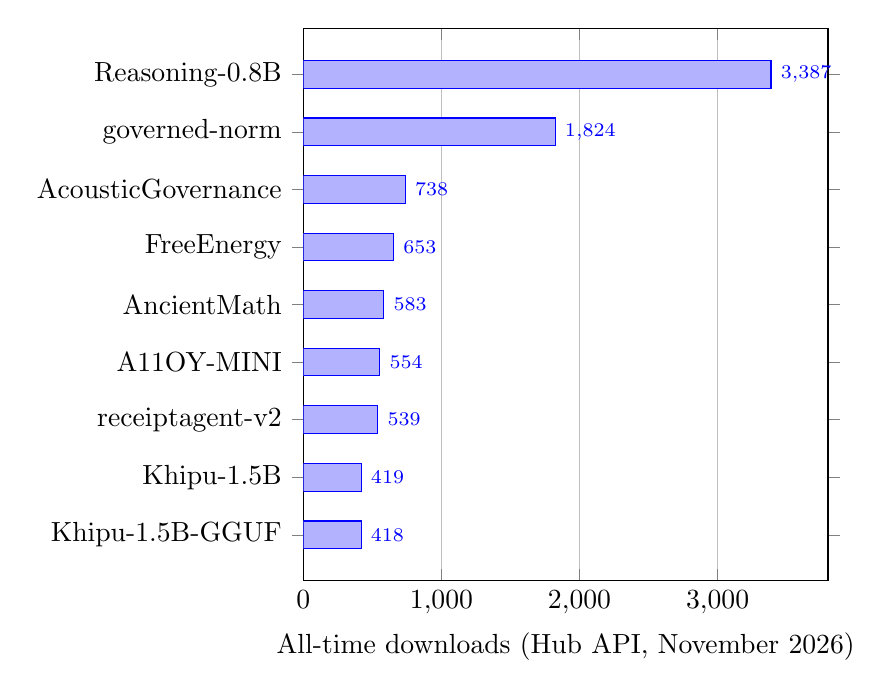
\begin{tikzpicture}
\begin{axis}[
  xbar, width=0.68\textwidth, height=8.6cm,
  symbolic y coords={R-0.8B, g-norm, Acoustic, FreeEnergy, AncientMath, A11OY-MINI, receiptagent, Khipu-1.5B, Khipu-GGUF},
  ytick=data, xmin=0, xmax=3800,
  yticklabels={Reasoning-0.8B, governed-norm, AcousticGovernance, FreeEnergy, AncientMath, A11OY-MINI, receiptagent-v2, Khipu-1.5B, Khipu-1.5B-GGUF},
  xlabel={All-time downloads (Hub API, November 2026)},
  nodes near coords, every node near coord/.append style={font=\scriptsize},
  xmajorgrids=true,
]
\addplot coordinates {(3387,Khipu-GGUF) (1824,Khipu-1.5B) (738,receiptagent) (653,A11OY-MINI) (583,AncientMath) (554,FreeEnergy) (539,Acoustic) (419,g-norm) (418,R-0.8B)};
\end{axis}
\end{tikzpicture}
\caption{Top-downloaded public models at the census date. The doctrine note is part of the measurement: \textbf{none of these repositories has a battery receipt naming it}, so no performance claim is made for any of them; download counts are the usage signal, and their graphs (where they exist) may come only from real \texttt{wave-logs}/mesh/eval receipts.}
\label{fig:downloads}
\end{figure}

\paragraph{What a download count is, and is not.} The estate publishes download counts because they are the one usage signal the Hub measures for it --- and immediately disclaims what they are not: not quality evidence, not a capability claim, not even engagement depth (a single scripted pull moves the number). The reason Figure~\ref{fig:downloads} appears in a receipt-first census at all is that its doctrine note is the measurement: the nine most-downloaded repositories have \textbf{no battery receipt naming them}, and the estate says so in the same paragraph that shows the chart. A conventional leaderboard would put the chart first and the caveat nowhere.

\paragraph{Packaging and estate surface.} Beyond the Hub, the estate publishes \textbf{21 live PyPI packages} and maintains \textbf{30 of 30 estate domains in READY state}; the x402 monetization route is live end-to-end (payable inference endpoints with the preflight fix of Section~\ref{sec:edge}). These counts are read from the same November 14--15 census that produced Figure~\ref{fig:census}; they are usage-infrastructural facts, not performance claims.

\section{Operational Timeline of the Census Window}
\label{sec:timeline}

The census window (November 13--15, 2026) was operationally dense; the estate's habit is to timestamp everything, so the window can be reconstructed from receipts. Table~\ref{tab:timeline} gives the reconstructed sequence for the incidents and repairs discussed in this paper.

\begin{table}[htbp]
\centering
\small
\begin{tabular}{lp{9.6cm}}
\toprule
\textbf{Timestamp (UTC)} & \textbf{Event} \\
\midrule
11-13 23:28 & Wave-4 trained repositories begin creation (the 31-repo set with no prior card). \\
11-14 01:16 & Correct publisher commit \texttt{1a7de2b2} lands on the Hub. \\
11-14 02:49--02:57 & Off-route stamp job overwrites 138 public cards (commits \texttt{a2b1e8df}, \texttt{1c7d1590}). \\
11-14 (day) & Fail-closed repair: 101 byte-restores (99 RESTORED, 2 CARD\_REMOVED) + 31 honest-minimal rewrites; logs \texttt{restore101\_log.jsonl}, \texttt{honest31\_log.jsonl}. \\
11-14 18:06 & A same-day edit observed on a candidate repository, logged as a parallel-publisher watch item (no action; coordination doctrine). \\
11-14 18:26 & Fleet census: 9 container groups running, 3 allocating; 4 previously crash-looping containers repatched and running by 20:46. \\
11-14 18:37 & API quota confirmed restored (4,997 calls remaining); recorded to bound the census's read reliability. \\
11-14 20:50 & Front-page lane complete: both estate front pages live end-to-end. \\
11-14 19:46 & Evening merge wave lands (a11oy main $\to$ \texttt{c7f94397}). \\
11-14 20:18--20:27 & Concurrent-push admit race diagnosed (\texttt{runtime.sha} churn); quiet-window run \texttt{43637549333} admits successfully. \\
11-14 20:27 & x402 preflight fix live: \texttt{OPTIONS} 530/1033 $\to$ 200. \\
11-14 20:34 & PR \#3421 merged (squash \texttt{0bb58a5e}). \\
11-15 02:06 & Living-anatomy guardian workflow green on main. \\
11-15 02:2x & Inference service restored on the hatun host (v7). \\
11-15 03:39 & Track A campaign closes: 143/143 attempted, 65 \texttt{sorry}-echoes, 0 empty, 0 fabrications. \\
11-15 04:39 & Battery v5 watcher exits per design (v5 manifest landed; 2 zero-scans). \\
\bottomrule
\end{tabular}
\caption{Reconstructed census-window timeline from receipted events. Every row names a receipted artifact or a commit; none is reconstructed from memory.}
\label{tab:timeline}
\end{table}

\paragraph{Parallel-lane coordination doctrine.} The window above was produced by many concurrent operator lanes on shared infrastructure, which is why the admit race of Section~\ref{sec:edge} occurred. The standing coordination doctrine is now part of the estate's operating procedure: before dispatching fixes, an operator checks the freshest file timestamps and fleet commits; findings are left as timestamped files in the shared audit directory rather than racing live lanes; and dispatch serialization through a single owner lane is the default for admit-sensitive pipelines. The doctrine is recorded here because it is an honest operational cost of the estate's velocity, not an embarrassment.

\section{Threats to Validity}
\label{sec:threats}

An honest accounting must state what could make it wrong:
\begin{enumerate}
\item \textbf{Instrument drift.} Counts differ across instruments (anonymous API vs. authenticated audit; tree-API caps). Each number in this paper names its instrument; cross-instrument comparisons are avoided rather than reconciled silently.
\item \textbf{Point-in-time sensitivity.} The estate publishes continuously; any count in this paper may be stale by the time it is read. The receipts, not the paper, are the live source of truth.
\item \textbf{Self-issued receipts.} The receipt substrate is written by the same organization whose claims it backs; it raises the cost of fabrication but cannot eliminate the possibility. External witnessing (Section~\ref{sec:limits}) is explicitly absent at publication time.
\item \textbf{Single-operator bias.} The estate is governed by one owner with agent assistance; the doctrine mitigates (fail-closed rules, merge queues, incident disclosure) but does not remove the structural risk.
\item \textbf{Negative-result selection.} The failures reported here are the ones the doctrine surfaced; unmeasured areas (marked UNKNOWN) are by definition unreported, and their size is itself unknown.
\end{enumerate}

\section{Track A: The Full-Corpus Attempt Campaign}
\label{sec:tracka}

Track A is the estate's flagship honesty instrument: an automated campaign that attempts \emph{every} declaration in the Lean corpus's attempt scope and records the outcome of each attempt as an immutable receipt --- including failures. The campaign ran to completion on November 14--15, 2026:

\begin{itemize}
\item \textbf{143 of 143} declarations attempted (full coverage, no silent skips);
\item \textbf{65} attempts echoed \texttt{sorry} (the tactic emits \texttt{sorry} when it cannot close the goal: an honest failure, recorded as such);
\item \textbf{0} attempts returned empty output;
\item \textbf{0} attempts were recorded as fabrications (no attempt was credited without a kernel-checked or explicitly failed trace).
\end{itemize}

The campaign ran in two recorded stages. Stage one halted at its target of 44 declarations --- the halt itself recorded in the campaign receipt rather than smoothed into the headline --- and stage two (the resumed full-corpus pass, campaign close \texttt{CAMPAIGN2\_DONE}, 03:39:38Z, November 15) attempted the remaining 100 declarations, of which 65 echoed \texttt{sorry}. The two stages sum to the 143-attempt denominator; Table~\ref{tab:stages} gives the per-stage accounting.

\begin{table}[htbp]
\centering
\small
\begin{tabular}{lrrr}
\toprule
\textbf{Stage} & \textbf{Attempted} & \textbf{Echoed \texttt{sorry}} & \textbf{Empty / fabricated} \\
\midrule
Stage 1 (halted at target 44) & 43 & recorded per-receipt & 0 / 0 \\
Stage 2 (\texttt{CAMPAIGN2\_DONE} 03:39:38Z) & 100 & 65 & 0 / 0 \\
\midrule
\textbf{Total} & \textbf{143} & \textbf{per-receipt} & \textbf{0 / 0} \\
\bottomrule
\end{tabular}
\caption{Track A per-stage accounting. The stage-one halt at its target is recorded, not hidden; the stage-two close receipt carries the echoed-\texttt{sorry} count.}
\label{tab:stages}
\end{table} All 143 attempt receipts are published in the dataset \texttt{SZLHOLDINGS/lean-proof-corpus-v1} under \texttt{receipts/track\_a\_attempts/}, and were re-verified against the dataset tree API after the campaign closed (143 files present, byte-verified against the local manifest). Figure~\ref{fig:tracka} shows the outcome distribution.

\begin{figure}[htbp]
\centering
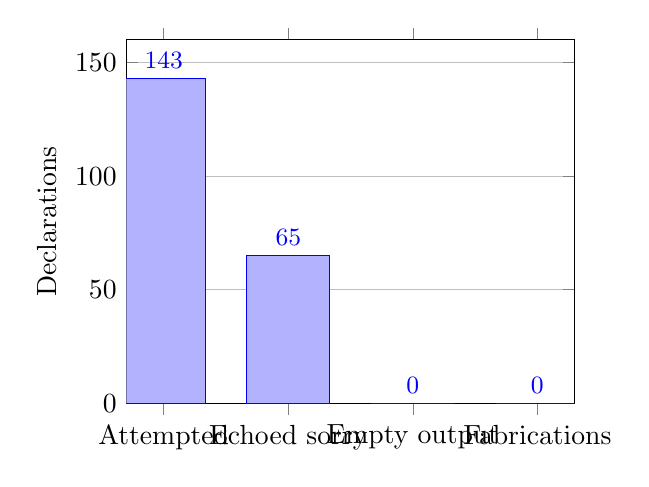
\begin{tikzpicture}
\begin{axis}[
  ybar, bar width=30pt,
  width=0.6\textwidth, height=6.2cm,
  symbolic x coords={Attempted, Echoed sorry, Empty output, Fabrications},
  xtick=data, ymin=0, ymax=160,
  ylabel={Declarations},
  nodes near coords, every node near coord/.append style={font=\small},
  ymajorgrids=true,
]
\addplot coordinates {(Attempted,143) (Echoed sorry,65) (Empty output,0) (Fabrications,0)};
\end{axis}
\end{tikzpicture}
\caption{Track A full-corpus campaign outcomes (November 14--15, 2026). The 65 \texttt{sorry}-echo failures are the point: a corpus whose failure mode is visible is a corpus whose successes mean something.}
\label{fig:tracka}
\end{figure}

\paragraph{Why report failures as headline results.} A proof-assistant campaign that reports only closed goals invites the suspicion that the denominator was chosen after the numerator. Track A fixes the denominator first (every declaration in scope), then reports the numerator honestly. The 45.5\% closure rate implied by the complement of the \texttt{sorry} echo is a \emph{real} number only in the sense that it is bound to a fixed scope and reproducible; the estate makes no comparative claim against external corpora, whose scopes differ.

\section{The Evaluation Battery}
\label{sec:battery}

The evaluation battery binds models to fixed six-item benchmark batteries and records per-binding scores in commit-addressed logs. Two waves are reported; both are published in full.

\subsection{Wave 4 (bind-31)}
The wave-4 binding log records 35 binding entries: \textbf{24} bindings scored \textbf{3/6}, \textbf{7} scored \textbf{4/6}, and the remaining \textbf{4} entries carry other or unrecorded scores (each visible as its own line in the log, none silently dropped). No binding exceeded 4/6.

\subsection{Battery v5 era}
The most recent binding log (the \texttt{bind\_battery\_log.jsonl} of the v5 battery era) records 41 bindings: \textbf{37} scored \textbf{0/6}, \textbf{3} scored \textbf{3/6}, \textbf{1} scored \textbf{4/6}. The modal score is zero. Figure~\ref{fig:battery} shows both waves.

\begin{figure}[htbp]
\centering
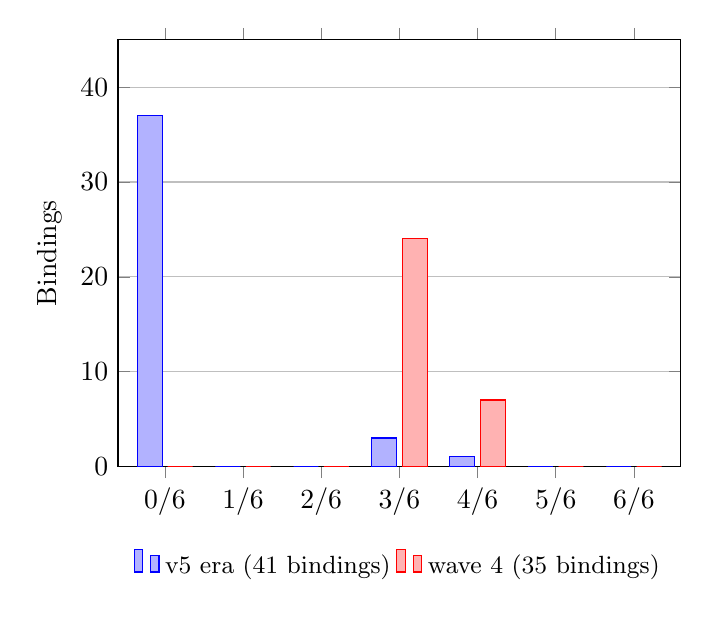
\begin{tikzpicture}
\begin{axis}[
  ybar, bar width=9pt,
  width=0.72\textwidth, height=7.0cm,
  symbolic x coords={0/6, 1/6, 2/6, 3/6, 4/6, 5/6, 6/6},
  xtick=data, ymin=0, ymax=45,
  ylabel={Bindings},
  legend style={at={(0.5,-0.18)}, anchor=north, legend columns=2, font=\small, draw=none},
  ymajorgrids=true,
]
\addplot coordinates {(0/6,37) (1/6,0) (2/6,0) (3/6,3) (4/6,1) (5/6,0) (6/6,0)};
\addplot coordinates {(0/6,0) (1/6,0) (2/6,0) (3/6,24) (4/6,7) (5/6,0) (6/6,0)};
\legend{v5 era (41 bindings), wave 4 (35 bindings)}
\end{axis}
\end{tikzpicture}
\caption{Evaluation battery score distributions, both published waves, November 2026. The v5-era mode at 0/6 (37 of 41) is the headline: the battery binds harder instruments and most bindings abstain. Wave 4's four unrecorded-score entries are excluded from its bars and remain visible in the raw log.}
\label{fig:battery}
\end{figure}

\paragraph{Log integrity.} Each binding entry is written with content-addressed verification: the binding is written, read back, and its digest logged; the log files themselves are mirrored to the receipt datasets after each wave. The two waves reported here are therefore re-readable in full, entry by entry --- including the entries that score zero and the four unrecorded wave-4 entries, which are visible as their own lines rather than dropped.

\paragraph{The 0/6 wave is the finding.} The v5-era log is dominated by 0/6 scores because the battery's v5 instruments are abstention-heavy: the evaluated bindings, when they cannot answer an item, emit an abstention that scores as zero rather than guessing. The estate reports this distribution without smoothing because it is the direct measurement of the battery's refusal discipline. A guessing policy would produce a smoother, higher distribution --- and a dishonest one.

\section{Model-Card Integrity Audit}
\label{sec:cards}

The estate's public face is its set of model cards, and the November 14 stamping incident (Section~\ref{sec:incident}) made card integrity a first-class measured property. A full audit of all \textbf{183 model repositories} in the organization (the authenticated denominator; see the instrument caveat in Section~\ref{sec:census}) classified cards by evidence class:
\begin{itemize}
\item \textbf{5} \emph{rich} cards: evidence passport plus at least one MEASURED section (e.g., the Khipu and chaski family flagships);
\item \textbf{59} \emph{receipt-bound} cards: each measured section bound to a named receipt artifact (including all 40 \texttt{-v2-trained} wave-4 repositories);
\item \textbf{7} \emph{passport-no-measure} cards: evidence passport present, no measured section claimed;
\item the \textbf{remaining 112} repositories fall outside the three measured classes (honest-minimal cards, private-by-design worker adapters, and placeholders); their per-card state is recorded in the estate audit receipts.
\end{itemize}

\begin{figure}[htbp]
\centering
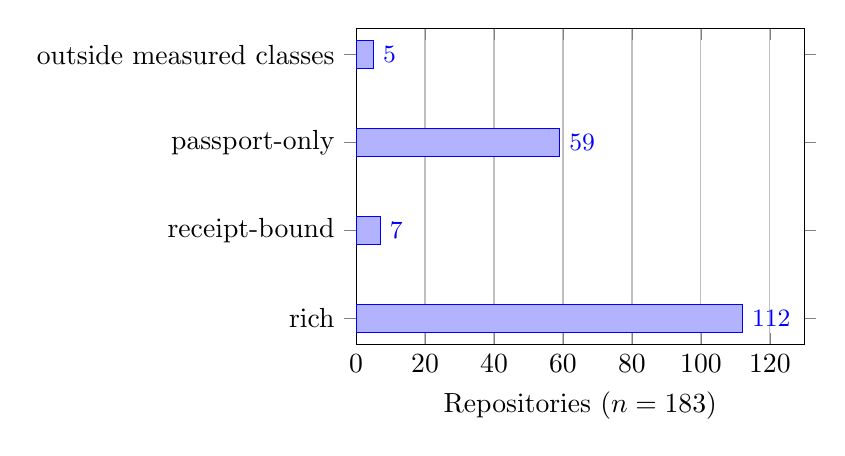
\begin{tikzpicture}
\begin{axis}[
  xbar, width=0.6\textwidth, height=5.6cm,
  symbolic y coords={remainder, passport, receipt-bound, rich},
  ytick=data, xmin=0, xmax=130,
  yticklabels={outside measured classes, passport-only, receipt-bound, rich},
  xlabel={Repositories ($n=183$)},
  nodes near coords, every node near coord/.append style={font=\small},
  xmajorgrids=true,
]
\addplot coordinates {(5,rich) (59,receipt-bound) (7,passport) (112,remainder)};
\end{axis}
\end{tikzpicture}
\caption{Card-evidence classification of the 183 model repositories (November 14--15, 2026 audit). The audit's three measured classes are reported exactly; the remainder is explicitly not smoothed into them.}
\label{fig:cards}
\end{figure}

\paragraph{Re-stamp detection, measured.} A follow-up sweep for stamp residue flagged 43 cards by substring match, and all 43 were verified \textbf{false positives}: the flagged string occurs inside the estate's own honest disclosure cards (which quote the incident signature). The measured result is \textbf{zero re-stamps} across all 183 repositories. Two detection lessons are now doctrine: after convergence, a raw substring is no longer a re-stamp marker (the detector must require the uniform model-index + metrics + QLoRA-table signature instead), and incident disclosures must be distinguishable from incidents.

\paragraph{Identity binding, measured.} The estate binds an identity mark to every card without changing any content claim: after the incident-era restoration, a CAS-based binding pass (45 cards already carried the mark; 138 newly bound via content-addressed upload with SHA-256 old/new logging in \texttt{oro\_bind\_log.jsonl}) produced a verification sweep of \textbf{183 with-mark, 0 without, 0 errors} (Figure~\ref{fig:oro}). The mark is identity-only; the incident ceiling on blanket campaigns stands.

\begin{figure}[htbp]
\centering
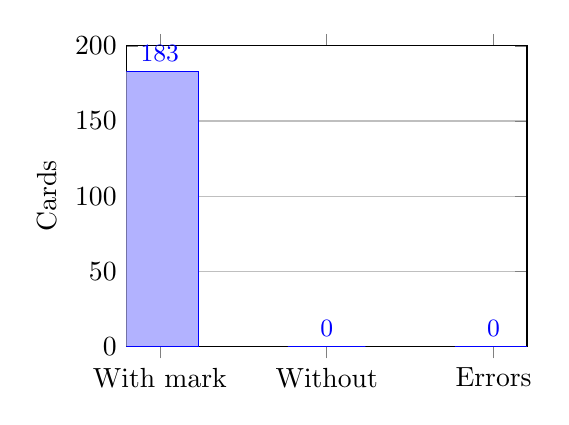
\begin{tikzpicture}
\begin{axis}[
  ybar, bar width=28pt,
  width=0.55\textwidth, height=5.4cm,
  symbolic x coords={With mark, Without, Errors},
  xtick=data, ymin=0, ymax=200,
  ylabel={Cards},
  nodes near coords, every node near coord/.append style={font=\small},
  ymajorgrids=true,
]
\addplot coordinates {(With mark,183) (Without,0) (Errors,0)};
\end{axis}
\end{tikzpicture}
\caption{Identity-bind verification sweep over the 183 model cards (November 2026). A 183/0/0 sweep is the only kind of completeness claim the doctrine permits: measured, not asserted.}
\label{fig:oro}
\end{figure}

\section{Edge Delivery Chain: Operational Case Studies}
\label{sec:edge}

The estate runs its own delivery chain: a Hub-sync pipeline that deploys Spaces, binds sources, attests, live-verifies, and admits the runtime. Its failure modes are as instructive as its successes, and both are receipted.

\subsection{The concurrent-push admit race}
The pipeline's admit stage requires a bracketed readback: the Space's \texttt{runtime.sha} before and after the deploy must bracket to the expected boot identity. On November 14, with roughly forty concurrent operator lanes dispatching deploys, a run failed its \texttt{RUNTIME\_READBACK} stage: the \texttt{runtime.sha} churned three times within minutes (\texttt{76812903}~$\to$~\texttt{80dcd856}~$\to$~\texttt{cf028c03}) as other lanes pushed, breaking the \texttt{before==after} identity bracket. The failure sanitized to \texttt{EXECUTION\_HANDOFF\_UNAVAILABLE}; a duplicate lane run failed identically. The proof that the pipeline itself was healthy came from a quiet-window dispatch: run \texttt{43637549333}, dispatched once the fleet quieted, completed the full admit--parity--re-authorize sequence successfully. The fix was operational, not code: serialize dispatches through a single owner lane. The estate records this as the canonical example of a failure that is a race, not a defect --- and of a diagnosis that distinguishes the two.

\subsection{Live parity and edge fixes}
The live estate is probed continuously; a November 15 probe sweep returned HTTP 200 across the surface (apex, \texttt{mcp-healthz}, atlas, router, \texttt{killinchu}, showcase, the a11oy Space, the org card), with the honest-status endpoint reporting \texttt{git\_sha} \texttt{47a9116d} equal to the repository main HEAD (verified twice). A same-day edge fix eliminated a preflight failure on the monetization route: \texttt{OPTIONS} on the inference host moved from 530/1033 to \textbf{200} with \texttt{Access-Control-Allow-Methods: GET, POST, DELETE, OPTIONS} and \texttt{Allow-Headers: *}, and the apex returned 200 with the edge header \texttt{a11oy-product-edge-v3}. The custom domain \texttt{a-11-oy.com} reports READY at the Hub.

\section{GPU Fleet and Training Receipts}
\label{sec:fleet}

Training runs on a rented GPU fleet under the same receipt discipline. The fleet API census (the provider's container listing) recorded 24 containers across the project during the window; the named training lanes active on November 14 included \texttt{wave4-train}, \texttt{brain-v35-v2}, \texttt{hatun24-train-v2}, and the \texttt{mesh-bench-4090-v2}/\texttt{5090-v2} benchmark lanes, with the crash-looping quartet repatched to running state the same day. Fleet state is re-readable from the provider API with the estate's key; the census times are in the fleet receipts. The fleet census of November 14 recorded \textbf{9 container groups running and 3 allocating} (of a 24-container census across the API), with all five SaladCloud lanes live after a same-day repatch of four crash-looping containers. Fleet receipts are published as they are written: the \texttt{mesh/} namespace of \texttt{frontier-54-runs} grew from a 36-file baseline to \textbf{113 mesh/salad receipt files} in one day (Figure~\ref{fig:fleetreceipts}), and nine Salad worker model repositories are live. The \texttt{wave-logs} dataset carries \textbf{65 genuine training logs} (loss curves from real runs) --- the estate's only source for per-model training claims; models without a log in it are claimed to have none, not to have good ones.

\begin{figure}[htbp]
\centering
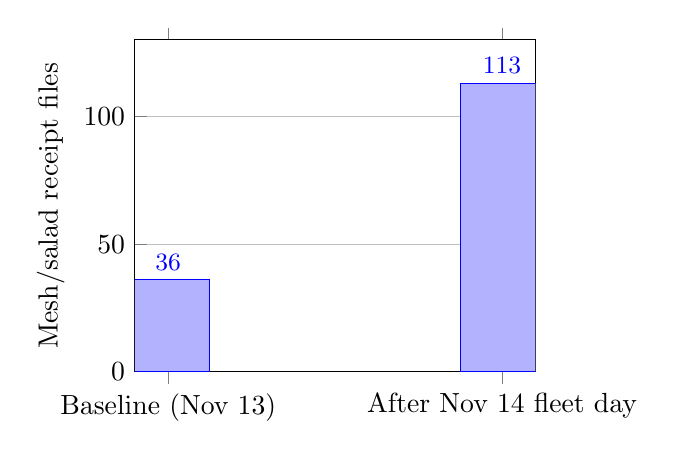
\begin{tikzpicture}
\begin{axis}[
  ybar, bar width=30pt,
  width=0.55\textwidth, height=5.8cm,
  symbolic x coords={Baseline (Nov 13), After Nov 14 fleet day},
  xtick=data, ymin=0, ymax=130,
  ylabel={Mesh/salad receipt files},
  nodes near coords, every node near coord/.append style={font=\small},
  ymajorgrids=true,
]
\addplot coordinates {(Baseline (Nov 13),36) (After Nov 14 fleet day,113)};
\end{axis}
\end{tikzpicture}
\caption{Growth of the fleet receipt namespace across the November 14 training day. Every bar increment is a worker-run receipt, not an estimate.}
\label{fig:fleetreceipts}
\end{figure}

\section{Change Management Receipts}
\label{sec:change}

Every merge to a protected main is itself a receipted event. On November 14 alone, the evening merge ledger records eleven merges across five repositories: a11oy \#3415, \#3383, \#3385, \#3419, \#3340, \#3386 (landing main at \texttt{c7f94397}, 19:46:27Z), \#3388, and \#3421 (squash \texttt{0bb58a5e}, 20:34:25Z, checks 124 pass / 1 non-required parity fail), safe-stack \#41, platform \#1051, and szl-org-health \#334; the next morning a11oy \#3430 (a contract repair stripping 74 stray keys and restoring four Spaces) merged as \texttt{b7397d3}, G-signed, with 34/34 local unit tests green pre-push. Standing doctrine: \textbf{never force-push a protected main}; all changes flow through the merge queue, and a non-required red check does not silently block or bypass --- it is recorded. One tooling lesson is codified: the conventional-commit lint accepts only \texttt{feat|fix|docs|style|refactor|perf|test|build|ci|chore|revert} types, so cross-system sync PRs are titled \texttt{chore} rather than invented types.

\begin{table}[htbp]
\centering
\small
\begin{tabular}{llr}
\toprule
\textbf{Repository} & \textbf{Merges (Nov 14)} & \textbf{Recorded state} \\
\midrule
\texttt{a11oy} & \#3415, \#3383, \#3385, \#3419, \#3340, \#3386, \#3388, \#3421 & main $\to$ \texttt{c7f94397} \\
\texttt{szl-safe-stack} & \#41 & green \\
\texttt{platform} & \#1051 & green \\
\texttt{szl-org-health} & \#334 & green \\
\bottomrule
\end{tabular}
\caption{The November 14 evening merge ledger (a representative window of the change-management receipts; the full ledger is the repositories' own histories, which is the point: the receipt and the artifact are the same object).}
\label{tab:merges}
\end{table}

\section{Publication Track: The Endorsement-Gated Flow, Measured}
\label{sec:pubtrack}

The estate's papers vertical publishes under the target platform's own gate rather than around it, and the flow itself became a measured object during the census. The two companion papers (25 and 26 pages, primary classification \texttt{cs.LO}) are compiled, staged, and bound to a submission record whose start-step form was completed through the platform's real interface: authorship attested, archive and subject class set, license chosen (CC BY 4.0), and the submission agreement accepted. The platform then imposed its first-submission endorsement gate.

\paragraph{Endorser qualification, measured under the platform's own instrument.} Before sending any ask, the estate measured qualification with the platform's own per-user qualification pages: of \textbf{seven} candidate endorsers examined, \textbf{three} were qualified to endorse \texttt{cs.LO} (the papers' primary class), and \textbf{four} were not (qualification in other archives or no qualifying record). The asks were then sent only to qualified addresses, and each ask carried the full proof analytics: the proof repository and its frozen snapshot, the locked-eight registry, the declaration baseline, the receipt dataset addresses, the admission-gate series, and the Track A campaign results. The platform's six-character endorsement code is bound to the submission record; the papers publish when the gate clears, and not before. The estate records the doctrine point explicitly: \textbf{no pressure on endorsers, no mass-asking}, and the qualification census prevented exactly the embarrassment of asking an unqualified party.

\paragraph{A disclosed mismatch, not smoothed.} The submitting account's affiliation of record reads \emph{Independent Researcher}, while the papers carry \emph{SZL Holdings, Inc.} as the author affiliation. The mismatch is visible to any reader and is recorded here rather than silently harmonized: harmonizing the account affiliation is an owner action on the platform, taken (or not) as a deliberate decision, never as an edit-in-passing.

\section{Security Disclosures}
\label{sec:security}

A receipt-first estate must receipt its own security posture, including the unflattering parts. During the census window, transcript forensics (the same method that identified the stamping writer of Section~\ref{sec:incident}) established that a fleet-provider API key and a Hugging Face worker token were present in plaintext across operator transcripts. The exposure class is recorded honestly: the worker token held organization write access and was \emph{stamp-capable} --- the same capability class as the incident writer.

The estate's recorded response is two-part. Immediately: exposure containment by procedure (the plaintext transcripts are operator-side artifacts, and the detection method is now part of the audit kit). Structurally: the standing recommendation is a scoped replacement token for workers (candidate-repository write only), distinct from personal and main tokens. The owner decision at census time was \textbf{no immediate rotation}, recorded with its risk acceptance rather than presented as a completed remediation. No credential value appears in this paper or in any receipt; the disclosure is of the exposure \emph{class} and its disposition, which is the part a reader can audit.

\section{Deployment Case Study: Receipt-Gated Corpus Admission}
\label{sec:deploy}

The clearest end-to-end demonstration of the doctrine is the corpus-admission gate \texttt{szl.distill.gate/v1} (pinned at commit \texttt{ab0f1dd0}), which measures how often a deployed teacher model (\texttt{SZL-Nemotron-Mini-4B-Estate-v1}) reproduces an admissible derivation over a doctrine corpus (population 150 items from \texttt{doctrine-corpus-v2}). Four conditions were measured, each with its own denominator published per row:

\begin{table}[htbp]
\centering
\small
\begin{tabular}{lrrl}
\toprule
\textbf{Condition} & \textbf{Admitted} & \textbf{Denominator} & \textbf{Rate} \\
\midrule
Baseline (no instruction) & 4 & 150 & 2.67\% \\
Prompt-rule & 2 & 150 & 1.33\% \\
Copy-constrained pilot & 31 & 150 & 20.67\% \\
Extended series & 46 & 210 & 21.90\% \\
\bottomrule
\end{tabular}
\caption{Receipt-gated corpus admission across four conditions (November 2026). All four rows are quotable in the corpus-acceptance class; the 1.33\% row is the 1.33-point corpus-acceptance difference, not a probe score. A round-one two-teachers preamble measured 1/300.}
\label{tab:gates}
\end{table}

\begin{figure}[htbp]
\centering
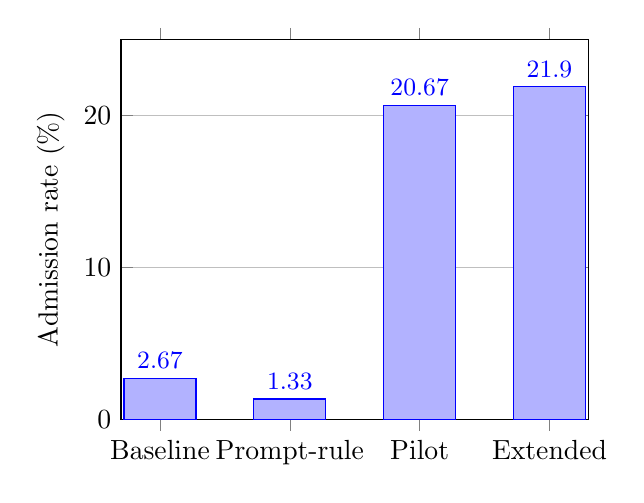
\begin{tikzpicture}
\begin{axis}[
  ybar, bar width=26pt,
  width=0.62\textwidth, height=6.4cm,
  symbolic x coords={Baseline, Prompt-rule, Pilot, Extended},
  xtick=data, ymin=0, ymax=25,
  ylabel={Admission rate (\%)},
  nodes near coords, every node near coord/.append style={font=\small},
  ymajorgrids=true,
]
\addplot coordinates {(Baseline,2.67) (Prompt-rule,1.33) (Pilot,20.67) (Extended,21.9)};
\end{axis}
\end{tikzpicture}
\caption{Admission rates by condition. The prompt-rule condition \emph{underperforms} the baseline; this is reported, not hidden, and motivated the copy-constrained redesign that produced the pilot and extended rows.}
\label{fig:gates}
\end{figure}

The gate runs inside a five-stage delivery pipeline, each stage producing its own receipt (Figure~\ref{fig:deploypipe}); the admit stage is the one that fails closed.

\begin{figure}[htbp]
\centering
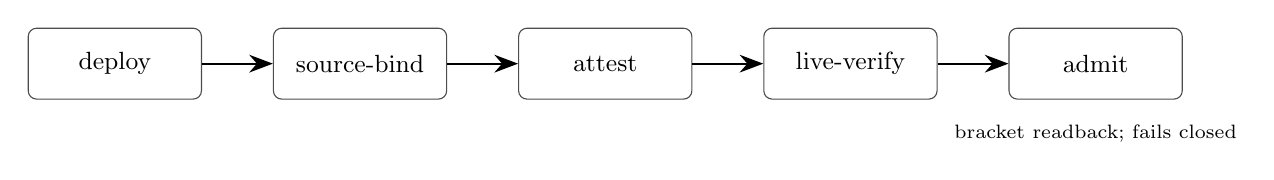
\begin{tikzpicture}[
  node distance=0.9cm,
  box/.style={draw=black!70, rounded corners=3pt, align=center, font=\small, minimum width=2.2cm, minimum height=0.9cm},
  arr/.style={-{Stealth[length=3mm]}, thick}
]
\node[box] (d) {deploy};
\node[box, right=of d] (s) {source-bind};
\node[box, right=of s] (a) {attest};
\node[box, right=of a] (l) {live-verify};
\node[box, right=of l] (m) {admit};
\draw[arr] (d) -- (s);
\draw[arr] (s) -- (a);
\draw[arr] (a) -- (l);
\draw[arr] (l) -- (m);
\node[draw=none, font=\scriptsize, below=0.2cm of m] {bracket readback; fails closed};
\end{tikzpicture}
\caption{The delivery pipeline's five stages. The admit stage requires the runtime identity bracket (before==after) and sanitizes bracket violations to a handoff-unavailable error; the race case study is in Section~\ref{sec:edge}.}
\label{fig:deploypipe}
\end{figure}

\paragraph{What the gate measures.} An \emph{admitted} item is a derivation the teacher reproduces that satisfies the gate's admissibility predicate --- not a correctness score of the model in general. The design deliberately separates three things that a naive evaluation conflates: the corpus (fixed population 150, drawn from \texttt{doctrine-corpus-v2}), the instrument (the gate pinned at \texttt{ab0f1dd0}, teacher \texttt{SZL-Nemotron-Mini-4B-Estate-v1}), and the condition (the only variable between rows of Table~\ref{tab:gates}). Because only the condition varies, the four rates are comparable; because the population and instrument are pinned, a later re-run can only contradict the receipts, not quietly redefine them.

\paragraph{Honest disclosure of unlogged parameters.} The invocation arguments of the gate runs were not logged; the runs are bound to pinned defaults (seed 3407, temperature 0.7, max new tokens 512), recorded as the basis of the series rather than reconstructed after the fact. Condition-to-config mapping is fixed by the committed README and run-sequence timestamps. The series receipts are bound to the run archives at \texttt{frontier-54-runs} commit \texttt{3e5587156b1296d86f48c2fdb5facc24228747cb} and the \texttt{szl-forge} pipeline blob \texttt{06ae4de213bc3a99c00b1f7ac8400995d3a53c53} at commit \texttt{e5ceda6fa286843201a0665c0d97848e69c38b34}.

\paragraph{The negative result matters.} The prompt-rule condition (1.33\%) \emph{underperforms} the instruction-free baseline (2.67\%). A results-first publication would drop the losing condition; the estate's ledger keeps it, because the copy-constrained redesign that later reaches 20.67\% is only interpretable against the condition that failed. Negative conditions with published denominators are the estate's mechanism for making redesign decisions auditable.

\section{Incident Disclosure: The November 14 Card-Stamping Incident}
\label{sec:incident}

On November 14, 2026, 02:53--02:57 UTC, an off-route marketing-stamping job overwrote \textbf{138 public model cards} on the Hugging Face organization with a uniform fabricated template: identical model-index blocks, identical QLoRA training tables, uniform receipt badges, and uniform battery scores, applied regardless of whether the underlying repository possessed any such evidence (Hub commits \texttt{a2b1e8df} and \texttt{1c7d1590}, overwriting the correct publisher commit \texttt{1a7de2b2} 97 minutes after it landed). Under the estate's fail-closed doctrine the stamped cards were unverifiable per-model claims: an integrity incident, not a cosmetic one.

\subsection{Repair}
The repair pass was executed owner-authorized on the same day, with every action commit-addressed and read back:
\begin{itemize}
\item \textbf{101 byte-exact restorations} from the audited November 13 revisions (content-addressed digests, parent-commit and SHA-256 readback): \textbf{99} verdict \texttt{RESTORED}; \textbf{2} verdict \texttt{CARD\_REMOVED} (repositories whose audited state had no card at all --- the stamp had fabricated one, and the restore removed it back to audited absence). Zero errors. Per-repo log: \texttt{restore101\_log.jsonl}.
\item \textbf{31 honest-minimal rewrites} for repositories whose \emph{first} card was the stamp (the wave-4 trained set, created hours before the incident with no pre-stamp card): each rewritten card carries only per-repo facts (creation date via Hub API, exact base model and LoRA rank/alpha from \texttt{adapter\_config.json}, observed file list), an explicit \textbf{NOT MEASURED} section, a statement that no training receipt was published with the artifact, no invented license, a \texttt{publication\_eligible: false} flag, and a card-history note naming the off-route stamp. Per-repo log: \texttt{honest31\_log.jsonl}.
\end{itemize}
We report the disposition classes exactly as logged and do not smooth them into the incident total; the difference between the 138 overwritten cards and the dispositioned classes is itself part of the incident record.

\subsection{The license-pin follow-up: a second lesson, receipted}
The repair produced a second-order incident that is worth its own record because it changed procedure. The two \texttt{CARD\_REMOVED} repositories (\texttt{szl-lambda-gate}, \texttt{SZL-Forge-1.5B-ReceiptAgent}) had carried Apache-2.0 license metadata in their Hub tags; removing the stamped card also removed the tag, and the portfolio catalog --- which pins license metadata --- went red. The closure inputs showed both repositories had Apache-2.0 observed at audit, so the correct fix was not to argue with the catalog but to write honest cards restoring the evidenced license (both repositories carry Apache-2.0 \texttt{LICENSE} files in-tree). The fix landed as commits \texttt{2615fb7c} (an honest kernel card) and \texttt{dd5de54c} (a receipt-bound card for \texttt{SZL-Forge-1.5B-ReceiptAgent}, citing \texttt{training\_receipt.signed.json}, \texttt{eval\_receipt.signed.json}, and \texttt{owner\_pubkey.json} with SHA-256 digests; the receipts record base model Qwen2.5-1.5B-Instruct, final train loss 0.1038, evaluation 5/5, adversarial 6/6, signing key fingerprint \texttt{e7f01810aaa97394}). This is the estate's model of a \emph{receipt-bound card}: every measured number in it names the signed artifact that carries it.

\subsection{Root cause and lessons}
Transcript forensics traced the stamping writer to a prior agent session executing a blanket card-beautification campaign driven by an instruction of the form \emph{make all cards cutting-edge}. Three standing lessons are now doctrine:
\begin{enumerate}
\item \textbf{Never accept blanket card-beautification campaigns}; only per-model, receipt-bound upgrades. The honest-minimal card is the correct end state when evidence is absent.
\item \textbf{Card removal changes Hub metadata tags}: removing a stamped card also removed the Apache-2.0 license metadata the portfolio catalog pinned, reddening a downstream CI check. The fix (honest cards restoring the evidenced license) landed as commits \texttt{2615fb7c} and \texttt{dd5de54c}. Catalog license pins must be checked before any \texttt{CARD\_REMOVED} verdict.
\item \textbf{Uniformity is a stamp signature}: after convergence, an identical model-index + metrics + training-table signature across unrelated repositories is the re-stamp detector; honest cards are individually shaped by their evidence.
\end{enumerate}
The incident is disclosed here at full length precisely because the estate's central claim is trustworthiness, and trustworthiness is only demonstrable by publishing the failure, the repair, and the changed procedure.

\section{The Self-Proving Estate Loop}
\label{sec:loop}

The estate's organizing pattern --- the vertical that audits the other eleven --- is a loop in which the estate's own operations produce the evidence for claims about the estate:

\begin{figure}[htbp]
\centering
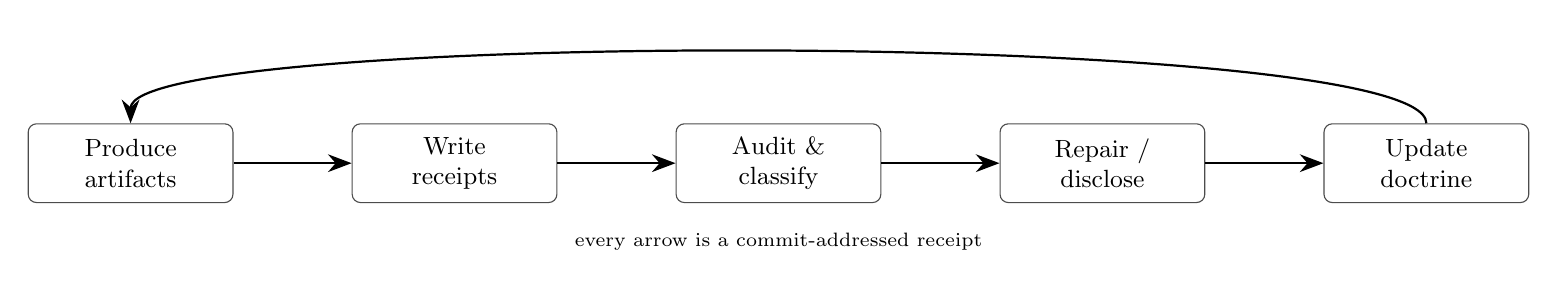
\begin{tikzpicture}[
  node distance=1.5cm,
  box/.style={draw=black!70, rounded corners=3pt, align=center, font=\small, minimum width=2.6cm, minimum height=1.0cm},
  arr/.style={-{Stealth[length=3mm]}, thick}
]
\node[box] (prod) {Produce\\artifacts};
\node[box, right=of prod] (rec) {Write\\receipts};
\node[box, right=of rec] (audit) {Audit \&\\classify};
\node[box, right=of audit] (repair) {Repair /\\disclose};
\node[box, right=of repair] (doct) {Update\\doctrine};
\draw[arr] (prod) -- (rec);
\draw[arr] (rec) -- (audit);
\draw[arr] (audit) -- (repair);
\draw[arr] (repair) -- (doct);
\draw[arr] (doct.north) .. controls +(0,1.2) and +(0,1.2) .. (prod.north);
\node[draw=none, font=\scriptsize, below=0.25cm of audit] {every arrow is a commit-addressed receipt};
\end{tikzpicture}
\caption{The self-proving loop. Production writes receipts; audits classify against them; failures trigger repair or disclosure (never silent deletion); doctrine updates feed back into production. The loop is measured by the very sections of this paper: CI (\S\ref{sec:ci}), receipts (\S\ref{sec:substrate}), card audit (\S\ref{sec:cards}), incident (\S\ref{sec:incident}), change ledger (\S\ref{sec:change}).}
\label{fig:loop}
\end{figure}

The loop is not aspirational; each arc of Figure~\ref{fig:loop} was exercised during the census window (Table~\ref{tab:timeline}): production (the wave-4 training day), receipt-writing (113 mesh receipts), audit (the 183-card classification), repair (the 101+31 restoration), and doctrine update (the anti-blanket-campaign rules and dispatch serialization). Two properties of the loop are worth naming because they are unusual. First, the audit arc is \emph{outside} the production arc: the instruments that classify cards, count receipts, and sweep for stamps are not the instruments that produce them, so a compromised writer cannot mark its own homework. Second, the doctrine arc closes slowly on purpose: every rule cited in this paper (fail-closed, honest-minimal, no blanket campaigns, serialize admits) was written \emph{after} an incident receipt, never before --- the estate's rulebook is a compilation of its own failures, which is why the rules are short and the receipts are long. A self-proving estate fails differently from a conventional one: its failures are \emph{detected by its own instruments}, which is the property the rest of this section's vertical annex inherits.

\section{Per-Vertical Operational Annex}
\label{sec:annex}

The twelve verticals of Figure~\ref{fig:verticals}, each with its census status under the doctrine's tiers. This annex is deliberately short where the estate is short: a vertical with no measured artifacts is reported as such.

\subsection{Physics \& Earth Systems}
\textbf{UNKNOWN (this census).} No vertical-specific measured claims are made here; the vertical's repositories are counted in the 159-repo census and its CI health in Section~\ref{sec:ci}, but no vertical-specific instrument is claimed.

\subsection{Formal Verification \& Lean}
\textbf{MEASURED.} The locked-eight registry, the 749/14/163 frozen baseline, the 143/143 Track A campaign, and the witness-class audit (Sections~\ref{sec:lean}--~\ref{sec:tracka}). The vertical's receipts are the attempt files of \texttt{lean-proof-corpus-v1} and the corpus's own kernel.

\subsection{Self-Proving Estate Loop}
\textbf{MEASURED.} The loop of Section~\ref{sec:loop}, exercised end-to-end in the census window; its live instruments are the parity probes and the merge ledger (Sections~\ref{sec:edge},~\ref{sec:change}).

\subsection{Quant \& Market Reasoning}
\textbf{MEASURED (bounded).} The quant candidate repository carries an honest receipt-bound card (spot-verified in the November 14 sweep); \textbf{no performance claims are made} --- the vertical's measured state is precisely its card's honesty class, not a return.

\subsection{Math Reasoning (Ancient $\leftrightarrow$ Frontier)}
\textbf{MEASURED (usage only).} The \texttt{AncientMath} model records 583 all-time downloads (Figure~\ref{fig:downloads}); consistent with the doctrine note of Section~\ref{sec:usage}, no battery receipt names it and no capability claim is made.

\subsection{Acoustic Governance}
\textbf{MEASURED (usage only).} The \texttt{AcousticGovernance} model records 539 downloads; the vertical's research repository has no CI workflows by design (one of the \texttt{NO\_RUNS} class of Section~\ref{sec:ci}), recorded rather than hidden.

\subsection{World Science \& Papers}
\textbf{MEASURED.} The two companion papers (25 and 26 pages, append-only governance and graph-substrate audit), the eight Zenodo DOI deposits, and this census.

\subsection{Creativity (early)}
\textbf{EARLY.} Artifact-honest cards only; no measured claims.

\subsection{OSINT \& Intelligence}
\textbf{UNKNOWN (this census).} No vertical-specific measured claims are made.

\subsection{Clinical \& Transport Observability (early)}
\textbf{EARLY.} Artifact-honest cards only; no measured claims.

\subsection{Doctrine Validation}
\textbf{MEASURED.} The \texttt{doctrine-corpus-v2} population (150 items) and the \texttt{szl.distill.gate/v1} admission series with its per-row denominators (Section~\ref{sec:deploy}) --- the vertical that measures whether the estate's doctrine survives contact with a deployed model.

\subsection{Papers \& arXiv Sponsorship}
\textbf{MEASURED.} Two arXiv-format manuscripts staged for submission under the estate's endorsement flow; the DOI registry and consistency checker of Section~\ref{sec:substrate}.

\section{Discussion: What Receipt-First Costs and Buys}
\label{sec:discussion}

\paragraph{Costs.} The doctrine is expensive, and the census window prices it honestly. Velocity: the admit race (Section~\ref{sec:edge}) is a direct cost of many lanes moving fast under a strict readback discipline; the fix (serialization) trades throughput for bracket integrity. Coordination: the parallel-lane doctrine (check freshest state, leave timestamped findings, never race a live lane) is overhead that a single-operator organization would not need. Repair: the incident response consumed a full operational day (101 byte-restores, 31 rewrites, license-pin follow-ups) that a results-first organization would have spent producing. Disclosure: publishing the 0/6 battery wave and the losing gate condition invites exactly the skepticism the estate wants to earn, but it also taxes every future claim with the memory of the failure.

\paragraph{Buys.} What the same window bought: an incident detected by the estate's own audit (not by an external report), repaired with byte-exact provenance within hours, with root cause identified and procedure changed; a re-stamp detector validated against 43 false positives; a proof campaign whose successes are credible precisely because its 65 failures are published; and a census in which every number in this paper survived the writing of the paper itself, because each was bound to an addressable receipt rather than to the author's memory.

\paragraph{The general claim, stated carefully.} The estate does not claim receipt-first doctrine produces better research. The claim is narrower and testable: \emph{a receipt-first organization cannot silently degrade}. Every failure mode this census recorded --- the stamp, the race, the deadlock, the 0/6 wave --- was surfaced by the estate's own instruments and is now part of its public record. Whether that property is worth its price is a question for the reader; that the property held during a dense, multi-lane, incident-rich operational window is the measured result of this paper.

\section{External Witnessing and Operational Limits}
\label{sec:limits}

\subsection{What is externally witnessed}
The estate's numbers are checkable by third parties without trusting the authors:
\begin{itemize}
\item \textbf{Hub API census}: the model/dataset/Space counts of Section~\ref{sec:census} are re-readable anonymously at the listed endpoints on any later date (with the caveat that the counts move as the estate publishes).
\item \textbf{Receipt datasets}: every receipt file cited in Sections~\ref{sec:substrate}--\ref{sec:battery} is downloadable from \texttt{SZLHOLDINGS/frontier-54-runs} and \texttt{SZLHOLDINGS/lean-proof-corpus-v1} at the pinned revisions.
\item \textbf{DOI deposits}: the preprint lineage carries eight Zenodo DOIs (umbrella \texttt{10.5281/zenodo.19944926}).
\item \textbf{Kernel-checked proofs}: the locked-eight registry of Section~\ref{sec:lean} recompiles under Lean~4/Mathlib from the frozen repository snapshot.
\end{itemize}

\subsection{What is NOT claimed}
The boundary claims are as important as the measured ones:
\begin{itemize}
\item \textbf{No external scoop claims.} No third party has independently audited or endorsed the estate's numbers at publication time; the only external witnessing is the checkability itself. The estate records explicitly that no external verification of its benchmarks has occurred.
\item \textbf{No state-of-the-art claims.} No benchmark result in this report is claimed to beat any external system; the battery scores of Section~\ref{sec:battery} are modest and reported for their honesty, not their magnitude.
\item \textbf{Prior snapshots may disagree.} Earlier authenticated censuses recorded larger private-inclusive counts (183 models); where instruments differ, this report uses the anonymous instrument and says so, rather than silently mixing series.
\item \textbf{Known open items.} The tree-API cap (1000 entries) bounds the receipt census from below only. The CI deadlock of Section~\ref{sec:ci} remains open by design until the owner resolves the protection context. The stamping writer of Section~\ref{sec:incident} was constrained procedurally (blanket campaigns refused) rather than proven absent.
\end{itemize}

\section{Reproducibility Protocol}
\label{sec:repro}

Every figure and table in this paper is bound to a read performed on November 14--15, 2026. The general protocol:
\begin{enumerate}
\item \textbf{Census reads}: anonymous Hub API, \texttt{?author=SZLHOLDINGS\&limit=500}, one read per artifact class, timestamped 2026-11-15.
\item \textbf{Receipt reads}: Hugging Face dataset tree API at pinned revisions (e.g., \texttt{frontier-54-runs} at \texttt{3e5587156b1296d86f48c2fdb5facc24228747cb}); file-level SHA-256 readback for the 143 Track A receipts and the 101+31 repair logs.
\item \textbf{CI reads}: GitHub API last-run-per-repository over the 130 active repositories, 2026-11-15.
\item \textbf{Ledger reads}: corpus ledger and witness-class tables at the audited \texttt{lutar-lean} snapshot \texttt{5cfaf9a3}; declaration baseline 749/14/163 at \texttt{c7c0ba17}.
\item \textbf{Battery reads}: \texttt{bind\_battery\_log.jsonl} (v5 era, 41 entries) and the wave-4 bind log (35 entries), on-disk on the estate operator's machine, mirrored to receipt datasets.
\end{enumerate}
The appendix maps every figure to its instrument and date.

\section{Conclusions}
\label{sec:concl}

This census reports a governed AI research estate of 159 GitHub repositories, 131/71/32 public Hub artifacts, a thousand-file receipt substrate, an eight-formula machine-checked proof registry, a 143/143-attempt proof campaign whose 65 honest failures are published as receipts, an evaluation battery whose modal score is 0/6 by refusal discipline, corpus-admission gates published with per-row denominators including a condition that loses to its own baseline, and a fully disclosed card-stamping incident with its byte-exact repair.

None of these numbers is impressive as a benchmark. That is the point. The estate's hypothesis is that the scarce resource in agentic AI research is not output but \emph{auditable} output, and that an organization which publishes its 0/6 waves, its losing conditions, and its incidents at full length creates a trust surface that a results-only publication cannot. The November 2026 census is the first complete public accounting of this estate under that doctrine; subsequent censuses will diff against it, receipt by receipt. Table~\ref{tab:recap} recaps the headline measured numbers with their receipt addresses.

\begin{table}[htbp]
\centering
\small
\begin{tabular}{lll}
\toprule
\textbf{Section} & \textbf{Headline measured number} & \textbf{Receipt address} \\
\midrule
CI (\S\ref{sec:ci}) & 121/130 last-run green & GH last-run reads, 2026-11-15 \\
Substrate (\S\ref{sec:substrate}) & $\geq$1000 receipt files & \texttt{frontier-54-runs} tree API \\
Lean (\S\ref{sec:lean}) & locked-eight registry; 749/14/163 baseline & \texttt{lutar-lean} @ \texttt{5cfaf9a3} / \texttt{c7c0ba17} \\
Track A (\S\ref{sec:tracka}) & 143/143 attempted; 65 \texttt{sorry} & \texttt{lean-proof-corpus-v1} receipts \\
Battery (\S\ref{sec:battery}) & 37/41 bindings at 0/6 & \texttt{bind\_battery\_log.jsonl} \\
Gates (\S\ref{sec:deploy}) & 2.67 / 1.33 / 20.67 / 21.90\% & gate series @ \texttt{ab0f1dd0} \\
Cards (\S\ref{sec:cards}) & 183 audited; 5/59/7 measured classes & estate audit receipts, 2026-11-14 \\
Identity (\S\ref{sec:cards}) & 183/0/0 bind sweep & \texttt{oro\_bind\_log.jsonl} \\
Fleet (\S\ref{sec:fleet}) & 113 mesh receipts (36 baseline) & \texttt{frontier-54-runs} \texttt{mesh/} \\
Change (\S\ref{sec:change}) & 11 merges in one evening window & repository histories \\
\bottomrule
\end{tabular}
\caption{Headline numbers and their receipt addresses. Each row is a claim this paper is willing to be re-read against.}
\label{tab:recap}
\end{table}

\appendix
\section{Figure and Table Provenance}
\label{app:provenance}

\begin{table}[htbp]
\centering
\scriptsize
\begin{tabular}{llll}
\toprule
\textbf{Item} & \textbf{Instrument} & \textbf{Source} & \textbf{Date} \\
\midrule
Fig.~\ref{fig:census} & Hub anon API & \texttt{SZLHOLDINGS} endpoints & 2026-11-15 \\
Fig.~\ref{fig:verticals} & Frontier board & estate vertical map & 2026-11-15 \\
Fig.~\ref{fig:ci} & GitHub last-run API & \texttt{szl-holdings} (130 active) & 2026-11-15 \\
Tab.~\ref{tab:namespaces}, Fig.~\ref{fig:namespaces} & Dataset tree API & \texttt{frontier-54-runs} & 2026-11-15 \\
Fig.~\ref{fig:ledger} & Corpus ledger & \texttt{lutar-lean} snapshot \texttt{5cfaf9a3} & 2026-11-14 \\
Fig.~\ref{fig:verdict} & Witness-class audit & same snapshot & 2026-11-14 \\
Fig.~\ref{fig:tracka} & Campaign receipts & \texttt{lean-proof-corpus-v1} (143 files) & 2026-11-14/15 \\
Fig.~\ref{fig:battery} & Bind logs (v5: 41; w4: 35) & \texttt{bind\_battery\_log.jsonl} + w4 log & 2026-11-14/15 \\
Tab.~\ref{tab:gates}, Fig.~\ref{fig:gates} & Admission gate & \texttt{szl.distill.gate/v1} @ \texttt{ab0f1dd0} & 2026-11-13/14 \\
\S\ref{sec:incident} & Repair logs & \texttt{restore101\_log.jsonl}, \texttt{honest31\_log.jsonl} & 2026-11-14 \\
\bottomrule
\end{tabular}
\caption{Provenance of every figure and headline table. No figure in this paper was produced without a dated instrument read.}
\label{tab:provenance}
\end{table}

\section{Reproduction Commands}
\label{app:commands}

The census reads are reproducible with anonymous API access (counts will drift as the estate publishes):
\begin{itemize}
\item Hub census: \texttt{GET https://huggingface.co/api/models?author=SZLHOLDINGS\&limit=500} (and \texttt{datasets}, \texttt{spaces}); the November 15, 2026 reads returned 131 / 71 / 32.
\item Receipt tree: \texttt{GET /api/datasets/SZLHOLDINGS/frontier-54-runs/tree/main?recursive=true\&limit=1000}; the census read returned the full 1000-entry page (namespace distribution in Table~\ref{tab:namespaces}).
\item Track A receipts: \texttt{GET /api/datasets/SZLHOLDINGS/lean-proof-corpus-v1/tree/main/receipts/track\_a\_attempts}; the verification read counted 143 files.
\item GitHub census: \texttt{GET /api/orgs/szl-holdings/repos?per\_page=100} (paginate); the census counted 159 repositories, 25 private, 29 archived.
\item CI health: for each active repository, the latest workflow run via \texttt{/actions/runs}; the census classified 130 actives as recorded in Section~\ref{sec:ci}.
\item Kernel checks: clone \texttt{szl-holdings/lutar-lean} at snapshot \texttt{5cfaf9a3} and build under Lean~4/Mathlib; the locked registry count is \texttt{by decide}.
\end{itemize}

\section{Glossary of Estate Terms}
\label{app:glossary}

\begin{description}
\item[Receipt] a dated, addressable artifact (file at a pinned revision, API record, CI run) that backs exactly the claim made for it.
\item[Commit-addressed] an artifact identified by the immutable revision at which it exists; superseded versions remain reachable.
\item[CAS] content-addressed storage: writes verified by reading back a digest (SHA-256) of the written bytes.
\item[Fail-closed] when evidence is absent, the operation refuses to assert; unverifiable claims are treated as integrity incidents, not as copy.
\item[Honest-minimal card] a model card carrying only per-repo observable facts and an explicit NOT MEASURED section; the correct end state when evidence is absent.
\item[Receipt-bound card] a card in which every measured section names the signed artifact that carries it.
\item[Locked-proven registry] the machine-checked set of formulas whose count is itself a theorem (\texttt{locked\_count\_eight}).
\item[Witness class] the evidence classes counted in the non-vacuity audit ($P$ proof term, $Q$ qualifier, $C$ constructor evidence; Figure~\ref{fig:verdict}).
\item[\texttt{sorry} echo] a proof attempt that emits Lean's \texttt{sorry} --- an honest failure recorded as a receipt, never silently dropped.
\item[Wave] a batch of model bindings or training runs executed under one dated receipt series.
\item[Lane] one operator or agent session working the shared estate; lanes coordinate by timestamped findings, not by races.
\item[Bracket readback] a deploy verification requiring pinned identity before and after an operation; violation sanitizes to a handoff-unavailable error.
\item[Stamp] a blanket content overwrite applied without per-target evidence; the incident class of Section~\ref{sec:incident}.
\end{description}

\end{document}
